\documentclass[11pt]{exam}

\usepackage{amsmath, amssymb, multicol}
\usepackage{graphicx}
\usepackage{textcomp}
\usepackage{tikz}

\def\d{\displaystyle}
\def\b{\mathbf}
\def\R{\mathbb{R}}
\def\Z{\mathbb{Z}}
\def\N{\mathbb{N}}
\def\pow{\mathcal{P}}
\def\st{~:~}
\def\bar{\overline}
\def\inv{^{-1}}
\def\imp{\rightarrow}
\def\and{\wedge}


%\pointname{pts}
\pointsinmargin
\marginpointname{pts}
\addpoints
\pagestyle{head}
%\printanswers

\firstpageheader{Math 228}{\bf Practice Problems 2: Sets}{Spring 2012}


\begin{document}
\noindent \textbf{Instructions}: The problems below are purely for you to practice.  I will not collect these, but it is still a good idea to write out your solutions in full.  Any of these problems or problems similar are fair game for quizzes and exams.  

\begin{questions}
\question Let $A = \{1,2,3,4,5\}$, $B = \{3,4,5,6,7\}$ and $C = \{2,3,5\}$.
\begin{parts}
 \part Find $A \cap B$.
 \part Find $A \cup B$.
 \part Find $A \setminus B$.
 \part Is $C \subseteq A$?
 \part Is $C \subseteq B$?
\end{parts}

\question Let $A = \{x \in \N \st 3 \le x \le 13\}$, $B = \{x \in \N \st x \mbox{ is even}\}$, and $C = \{x \in \N \st x \mbox{ is odd}\}$.
\begin{parts}
  \part Find $A \cap B$.
  \part Find $A \cup B$.
  \part Find $B \cap C$.
  \part Find $B \cup C$.
\end{parts}


\question Find an example of sets $A$ and $B$ such that $A\cap B = \{3, 5\}$ and $A \cup B = \{2, 3, 5, 7, 8\}$.

\question Find an example of sets $A$ and $B$ such that $A \subseteq B$ and $A \in B$.

\question Recall $\Z = \{\ldots,-2,-1,0, 1,2,\ldots\}$ (the integers).  Let $\Z^+$ be the positive integers.  Let $2\Z$ be the even integers, $3\Z$ be the multiples of 3, and so on.
\begin{parts}
  \part Is $\Z^+ \subseteq 2\Z$?  
  \part Is $2\Z \subseteq \Z^+$?  
  \part Find $2\Z \cap 3\Z$.  Describe the set in words, and also in symbols (using a $\st$ symbol).
  \part Express $\{x \in \Z \st \exists y\in \Z (x = 2y \vee x = 3y)\}$ as a union or intersection of two sets above.
\end{parts}


\question Let $A_2$ be the set of all multiples of 2 except for $2$.  Let $A_3$ be the set of all multiples of 3 except for 3.  And so on, so that $A_n$ is the set of all multiple of $n$ except for $n$, for any $n \ge 2$.  Describe (in words) the set $\bar{A_2 \cup A_3 \cup A_4 \cup \cdots}$



\question Draw a Venn diagram to represent each of the following:
\begin{parts}
 \part $A \cup \bar B$
 \part $\bar{(A \cup B)}$
 \part $A \cap (B \cup C)$
 \part $(A \cap B) \cup C$
 \part $\bar A \cap B \cap \bar C$
 \part $(A \cup B) \setminus C$
\end{parts}

\newpage

\question Describe a set in terms of $A$ and $B$ which has the following Venn diagram:

\begin{center}
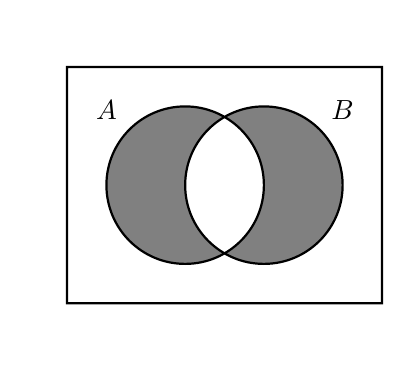
\begin{tikzpicture}[fill=gray]
% left hand
\scope
\clip (-2,-2) rectangle (2,2)
      (1,0) circle (1);
\fill (0,0) circle (1);
\endscope
% right hand
\scope
\clip (-2,-2) rectangle (2,2)
      (0,0) circle (1);
\fill (1,0) circle (1);
\endscope
% outline
\draw[thick] (0,0) circle (1) (-1,.7)  node [text=black,above] {$A$}
      (1,0) circle (1) (2,.7)  node [text=black,above] {$B$}
      (-1.5,-1.5) rectangle (2.5,1.5);
\end{tikzpicture}
\end{center}

\question Find the cardinalities:
\begin{parts}
  \part Find $|A|$ when $A = \{4,5,6,\ldots,37\}$
  \part Find $|A|$ when $A = \{x \in \Z \st -2 \le x \le 100\}$
  \part Find $|A \cap B|$ when $A = \{x \in \N \st x \le 20\}$ and $B = \{x \in \N \st x \mbox{ is prime}\}$
\end{parts}

\question Let $A = \{a, b, c\}$.  Find $\pow(A)$.

\question Let $A = \{1,2,\ldots, 10\}$.  How many subsets of $A$ contain exactly one element (i.e., how many {\em singleton} subsets are there).  How many {\em doubleton} (containing exactly two elements) are there?

\question Let $A = \{1,2,3,4,5,6\}$.  Find all sets $B \in \pow(A)$ which have the property $\{2,3,5\} \subseteq B$.

\question Find an example of sets $A$ and $B$ such that $|A| = 4$, $|B| = 5$ and $|A \cup B| = 9$.  

\question Find an example of sets $A$ and $B$ such that $|A| = 3$, $|B| = 4$ and $|A \cup B| = 5$.

\question If $|A| = 10$ and $|B| = 15$, what is the largest possible value for $|A \cap B|$?  What is the smallest?  What are the possible values for $|A \cup B|$?

\question If $|A| = 8$ and $|B| = 5$, what is $|A \cup B| + |A \cap B|$?

\question In a regular deck of playing cards there are 26 red cards and 12 face cards.  Explain in terms of sets why there are only 32 cards which are either red or a face card.

\question A group of college students were asked about their TV watching habits.  Of those surveyed, 28 students watch {\em House}, 19 watch {\em Castle} and 24 watch re-runs of {\em 24}.  Additionally, 16 watch {\em House} and {\em Castle}, 14 watch {\em House} and {\em 24} and 10 watch {\em Castle} and {\em 24}.  There are 8 students who watch all three shows.  How many students surveyed watched at least one of the shows?

\question Find $|(A \cup C)\cap \bar B|$ provided $|A| = 50$, $|B| = 45$, $|C| = 40$, $|A\cap B| = 20$, $|A \cap C| = 15$, $|B \cap C| = 23$ and $|A \cap B \cap C| = 12$.
%$|(A \cup C)\cap \bar B| = 46$

\question Using the same data as the previous question, describe a set with cardinality 26.
%One possibility: $(A \cup B) \cap C$.


\end{questions}




\end{document}


